\chapter{Fark Denklemleri}
Örnek sistemin ZOH yöntemi ile elde edilen ve Denklem~\ref{eqn:ornek_sistem_zoh} ile verilen sistem için
\begin{equation}
\begin{split}
    G_{ZOH}(z)&=\frac{1-e^{-1}}{z-e^{-1}}\\
    &=\frac{(1-e^{-1})z^{-1}}{1-e^{-1}z^{-1}}\\
    \frac{y(z)}{u(z)}&=\frac{(1-e^{-1})z^{-1}}{1-e^{-1}z^{-1}}\\
    y(z)(1-e^{-1}z^{-1})&=(1-e^{-1})z^{-1}u(z)\\
    y(z)-y(z-1)e^{-1}&=(1-e^{-1})u(z-1)\\
    y(z)&=y(z-1)e^{-1}+(1-e^{-1})u(z-1)\\
    y(z)&=0.3679y(z-1)+0.6321u(z-1)
\end{split}
\end{equation}
elde edilir. Z tanım bölgesinde tanımlı transfer fonksiyonundan fark denklemine geçişe örnektir. Fark denklemleri programlama dilleri ile kolaylıkla gerçeklenebilmektedir.
Benzer şekilde FOH yöntemi ile elde edilen ve Denklem~\ref{eqn:ornek_sistem_foh} ile verilen ifade için
\begin{equation}
    \begin{split}
        G_{FOH}(z)&=\frac{1}{z}\\
        \frac{y(z)}{u(z)}&=z^{-1}\\
        y(z)&=u(z-1)
    \end{split}
\end{equation}
elde edilir.
Yay-Kütle-Damper sistemi için dinamikleri ifade eden denklem
\begin{equation}
    m\ddot{x}(t)+b\dot{x}(t)+kx(t)=u(t)\label{eqn:mass_spring_damper}
\end{equation}
olarak verilmiştir. Bu diferansiyel denklem S tanım bölgesine dönüştürülürse
\begin{equation}
\begin{split}
    ms^2X(s)+b sX(s)+kX(s)&=U(s)\\
    (ms^2+b s+k)X(s)&=U(s)\\
    \frac{X(s)}{U(s)}=\frac{1}{ms^2+b s+k}
\end{split}
\end{equation}
elde edilir. Denklem~\ref{eqn:mass_spring_damper} ile verilen sistem için 
\begin{gather}
    m\frac{\Delta^2 x}{(\Delta t)^2}+b\frac{\Delta x}{\Delta t}+kx(kT)=u(kT)\nonumber\\
    m\frac{\Delta (x(kT)-x((k-1)T))}{kT-(k-1)T}+b\frac{x(kT)-x((k-1)T)}{kT-(k-1)T}+kx(kT)=u(kT)\nonumber\\
    m\frac{\Delta x(kT)-\Delta x((k-1)T)}{T^2}+b\frac{x(kT)-x((k-1)T)}{T}+kx(kT)=u(kT)\nonumber\\
    m\frac{x(kT)-2x((k-1)T)+x((k-2)T)}{T^2}+b\frac{x(kT)-x((k-1)T)}{T}+kx(kT)=u(kT)\nonumber\\
    m\frac{x(kT)-2x((k-1)T)+x((k-2)T)}{T^2}+b\frac{x(kT)-x((k-1)T)}{T}+kx(kT)=u(kT)\nonumber\\
    (m+bT+kT^2)x(kT)=(2m+bT)x((k-1)T)-mx((k-2)T)+T^2u(kT)\nonumber\\
    x(kT)=\frac{2m+bT}{m+bT+kT^2}x((k-1)T)-\frac{m}{m+bT+kT^2}x((k-2)T)+\frac{T^2}{m+bT+kT^2}u(kT)
\end{gather}
Örnek olması için $m=1\,kg$, $b=1\,Ns/m$, $k=1\,Nm$ ve $T=0.1$ olmak üzere fark denklemi
\begin{equation}
    x(kT)=1.8919x((k-1)T)-0.9009x((k-2)T)+0.009009u(kT)
\end{equation}
olarak elde edilir. Transfer fonksiyonundan yola çıkarak $\zeta=b\sqrt{m}/(2m\sqrt{k})$, $w_n=\sqrt{k}/\sqrt{m}$ ve $\phi=\cos^{-1}(\zeta)$ olmak üzere
\begin{equation}
\begin{split}
    G(z)&=\mathcal{Z}\left\{\frac{1-e^{-0.1s}}{s(s^2+s+1)}\right\}\\
    &=\frac{z-1}{z}\mathcal{Z}\left\{\frac{1}{s(s^2+s+1)}\right\}\\
    &=\frac{z-1}{z}\left(\frac{z}{z-1}-\frac{1}{\sqrt{1-\zeta^2}}\frac{\sqrt{1-\zeta^2}z^2+ze^{-\zeta w_nT}\sin(w_n\sqrt{1-\zeta^2}T-\phi)}{z^2-2ze^{-\zeta w_nT}\cos(w_n\sqrt{1-\zeta^2}T)+e^{-2\zeta w_nT}}\right)\\
    &=\frac{0.004833 z^3 - 0.0001585 z^2 - 0.004675 z}{ z^4 - 2.895 z^3 + 2.8 z^2 - 0.9048 z}\\
    &=\frac{0.004833 z + 0.004675}{z^2 - 1.895 z + 0.9048}
\end{split}
\end{equation}
elde edilir.
\begin{enumerate}
    \item Yay-kütle-damper sisteminin çıkış işaretini fark denklemlerini kullanarak elde ediniz. 
    \begin{lstlisting}
    m=1
    b=1
    k=1
    T=0.1
    fac1=(2*m+b*T)/(m+b*T+k*T**2)
    fac2=-m/(m+b*T+k*T**2)
    fac3=T**2/(m+b*T+k*T**2)
    tvec=np.arange(0,10+1,T)
    xt=np.zeros(tvec.shape)
    ut=np.ones(tvec.shape)
    for i in range(0,len(tvec)):
        if i==0:
            xt[i]=fac1*0+fac2*0+fac3*0
        elif i==1:
            xt[i]=fac1*xt[i-1]+fac2*0+fac3*ut[i-1]
        else:
            xt[i]=fac1*xt[i-1]+fac2*xt[i-2]+fac3*ut[i-1]

    plt.grid('minor')
    plt.xlabel("Zaman(s)")
    plt.ylabel("x(t)")
    plt.title("Yay-kutle-damper sistem yaniti")

    Gz=control.tf(1,np.array([m,b,k]))
    tc, yc=control.step_response(Gz)
    plt.plot(tc,yc,'k')
    plt.stem(tvec,xt,'b')
    plt.show()
    \end{lstlisting}

    \begin{figure}[!htb]
        \centering
        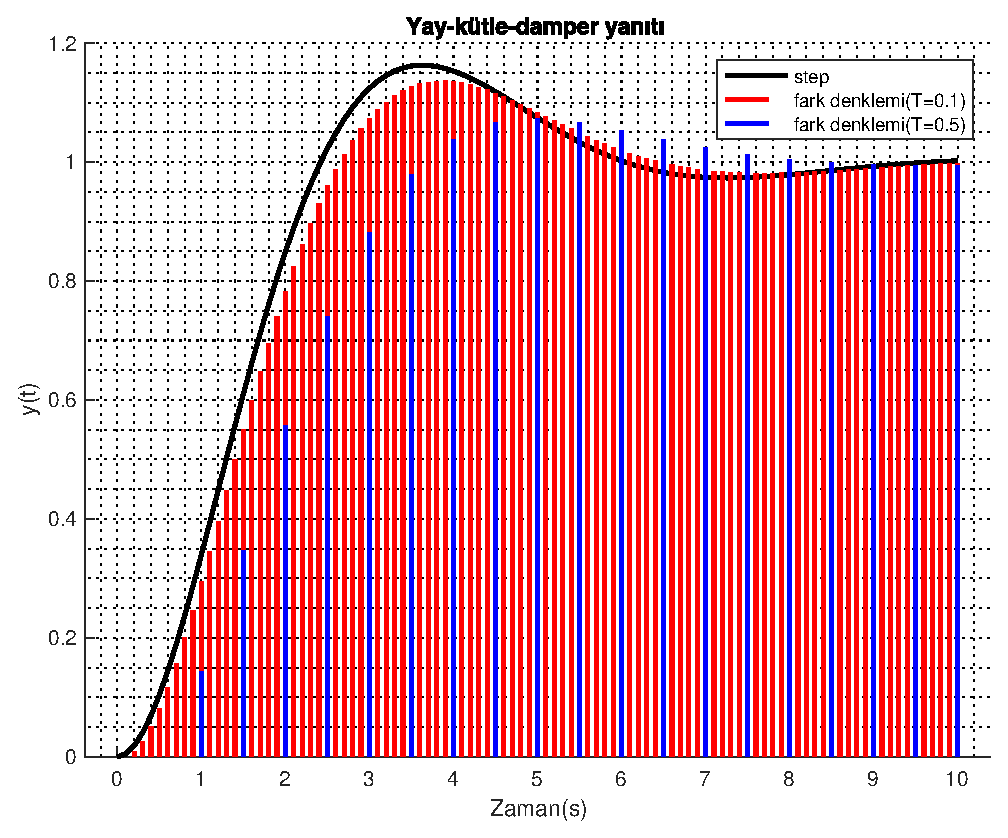
\includegraphics[width=0.5\textwidth]{img/lec3_step1}
        \caption{Yay-kütle-damper sisteminin çıkış işareti}
        \label{fig:lec3_step1}
    \end{figure}
    \item Yay-kütle-damper sisteminin çıkış işaretini ayrık transfer fonksiyonu kullanarak elde ediniz. 
    \begin{lstlisting}
    m=1
    b=1
    k=1
    
    plt.grid('minor')
    plt.xlabel("Zaman(s)")
    plt.ylabel("x(t)")
    plt.title("Yay-kutle-damper sistem yaniti")

    Gz=control.tf(1,np.array([m,b,k]))
    tc, yc=control.step_response(Gz)

    Gz1=control.c2d(control.tf(1,np.array([m,b,k])),0.1)
    tc1, yc1=control.step_response(Gz1)

    Gz2=control.c2d(control.tf(1,np.array([m,b,k])),0.5)
    tc2, yc2=control.step_response(Gz2)

    plt.plot(tc,yc,'k')
    plt.stem(tc1,yc1,'r')
    plt.stem(tc2,yc2,'b')
    plt.show()
    \end{lstlisting}
    \begin{figure}[!htb]
        \centering
        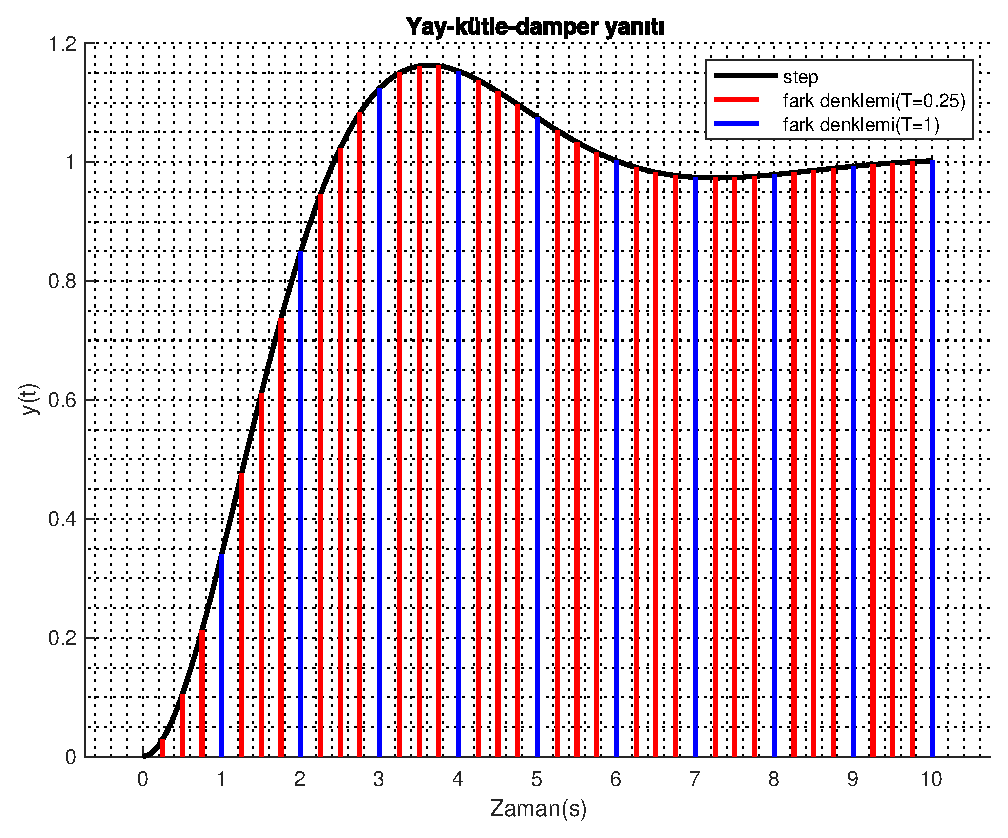
\includegraphics[width=0.5\textwidth]{img/lec3_step2}
        \caption{Yay-kütle-damper sisteminin çıkış işareti}
        \label{fig:lec3_step2}
    \end{figure}
\end{enumerate}